%Victor
\section{Suite de protocoles}
\label{sec:suiteprot}

\subsection{ARP} ARP (Address resolution protocol) est un protocole à cheval
entre la couche 2 et la couche 3 permettant de faire la conversion entre les
adresses de niveau 2 et de niveau 3. Il fut décrit dans le RFC 826\cite{url-RFC-ARP}.
Il est très utilisé étant donné que les hôte connaissent souvent les adresses
IP de leur destinataire, mais rarement l'adresse de niveau 2 de ce destinataire
ou de la passerelle à contacter pour joindre le destinataire.

\subsubsection{Cache ARP} Le cache ARP ou table ARP est une table stockée en
local par un hôte et qui ressence les associations entre adresses IP et adresses
MAC.  Ces associations peuvent être soit de type statique, donc écrite "en dur"
par l'administrateur, ou dynamique, donc issue d'échange de trame ARP, et qui
possèdent en plus, par rapport associations statique, une durée de validité, étant
donné qu'une interface peut changer d'adresse IP et qu'il faut maintenir la
table à jour.  Cette table peut donc être représentée comme une suite d'entrées,
contenant chacune une adresse IP, une adresse MAC et éventuellement une durée
de vie.

\subsubsection{Fonctionnement} Prenons l'exemple où un hôte A veux envoyer un message à
un hôte B. A connaît l'adresse IP de B. Donc A va préparer le paquet qu'il va envoyer
à B, avec son adresse IP en source et l'adresse IP de B en destination. Le
paquet passe dans la couche liaison, il va être empaqueté dans une trame de
niveau 2. Cette trame aura comme adresse source l'adresse de niveau 2 de A.
A ce moment là, il ne peux pas compléter l'adresse destination de la trame: en
effet, il ne connaît l'adresse de niveau 2 du destinataire. La paquet reste
bloqué en couche 2 et ne peux pas être envoyé au destinataire. Comment obtenir
l'adresse de niveau 2 du destinataire?  Le protocole ARP est capable de faire
cette translation.

Pour faire cela l'hôte A va tout d'abord regarder dans sa table ARP si il n'a
pas une entrée pour l'adresse IP à laquelle il souhaite envoyer son paquet. Si
il trouve une correspondance, il va utiliser l'adresse MAC stockée en
correspondance avec l'adresse IP recherchée.  Si il ne trouve pas de
correspondance il va émmetre une trame ARPREQUEST pour tenter de contacter le
possesseur de l'adresse IP qu'il souhaite contacter. Il va mettre dans cette
trame (en plus de l'entête de niveau 2) un entête ARP. Celui-ci contient entre
autre les adresses de niveau 2 et 3 de la source et du destinataire qui sont
essentiels pour faire la résolution d'adresse, ainsi qu'un champ qui spécifie
si la trame est un ARPREQUEST ou un ARPREPLY. 

\smallbreak
L'hôte A va donc mettre son
adresse IP en IP source (entête ARP) et son adresse MAC dans l'adresse physique
source (entête ARP). Dans le champ d'adresse IP destination (entête ARP) l'hôte
A va mettre l'adresse IP de l'hôte qu'il veut contacter. Etant donné qu'il
cherche à avoir l'adresse physique de l'hôte B, il ne peut pas indiquer
d'adresse de niveau 2 dans le champ d'adresse physique destinataire. Ce champ
est donc rempli avec la valeur 0 (entête ARP).  Sachant que l'hôte A n'a pas
l'adresse physique du destinataire, il va envoyer sa trame en broadcast pour
espérer atteindre l'hôte B sans connaître son adresse MAC. 
\smallbreak
Si l'hôte B reçoit
la requête ARP, il va analyser son entête et remplir sa table ARP avec
l'adresse IP de l'hôte A et l'adresse physique de A contenu dans l'entête ARP.
Cela permet de créer une correspondance entre l'adresse IP et l'adresse de
niveau 2 de A, pour non seulement pouvoir répondre à sa requête ARP, mais en
plus pouvoir contacter A dans le futur sans avoir besoin de refaire de requête
ARP. Ensuite l'hôte B va répondre avec une trame ARPREPLY. L'entête est
similaire aux ARPREQUEST, seul le champ indiquant s'il s'agit d'une trame
ARPREQUEST ou ARPREPLY change. Dans cette trame, l'hôte B va placer son adresse
IP dans le champ adresse IP source et son adresse physique dans le champ
d'adresse physique source de l'entête ARP. Il va aussi mettre l'adresse IP de A
dans le champ adresse IP destination et l'adresse MAC de A dans le champ
d'adresse physique destination (entête ARP).  Il va ensuite envoyer cette trame
en unicast à A.  Lorsque A reçoit la trame ARPREPLY, il va à son tour mettre
dans sa table ARP, la correspondance entre l'adresse IP source et l'adresse de
niveau 2 source de l'entête ARP (soit les adresses de B).  Une fois cette
association mise en place, le paquet IP que voulait envoyer A au début et qui a
été mis en pause le temps que le protocole ARP fasse l'association, est enfin
envoyé étant donné que A à maintenant l'adresse physique de B.


\subsubsection{ACD} Le protocole ACD (Adresse conflict detection) permet, comme
son nom l'indique, de détecter les conflits d'adresse, qui sont l'utilisation
de la même adresse IP par deux ou plusieurs hôtes en même temps. Pour ce faire
il utilise le protocole ARP avec une succession d'étape permettant de garantir
l'utilisation de manière unique d'une adresse IP. Il fut décrit dans le RFC
5227\cite{url-RFC-ACD}.
\smallbreak
Pour commencer, ACD intervient au moment où une interface reçoit une adresse IP
(soit par DHCP, soit par une configuration manuelle,...). Il faut à ce moment
vérifier si l'adresse proposée n'est pas déjà utilisée par un autre hôte sur le
réseau.  L'hôte va alors émettre une requête ARP en broadcast en remplissant
l'entête ARP avec son adresse de niveau 2 dans le champ d'adresse physique
source et 0.0.0.0 dans l'adresse IP source (car il n'a pas encore d'adresse IP
attribuée, et pour éviter de corrompre les tables ARP des autres hôtes). Le
champ adresse IP destinataire (entête ARP) est complété avec l'adresse que l'on
souhaite acquérir. On ne peut pas remplir le champ d'adresse physique
destinataire de l'entête ARP étant donné qu'on ne sait pas si il y a des hôte
avec cette adresse déjà configurée.  Une requête ARP contenant 0.0.0.0 comme
adresse IP source est appelée ARP probe car elle sert à "sonder" si un autre
hôte utilise déjà l'adresse que l'on passe dans le champ adresse IP
destinataire.

\smallbreak
Après avoir attendu un temps pouvant aller jusqu'à 1 seconde, l'hôte va envoyer
un nombre d'ARP probe compris entre 1 et 3, et tous espacé d'un intervalle
compris entre 1 et 2 secondes.  Si dans un délai de 2 secondes après l'émission
de l'ARP probe l'hôte reçoit une trame ARP request ou reply avec comme adresse
IP source (entête ARP) l'adresse qu'il souhaite acquérir, alors cela veut dire
qu'un autre hôte est déjà entrain d'utiliser cette adresse. L'ARP reply peut
être la réponse à un des ARP probe émis et l'ARP request peux simplement être
une demande ARP faite par l'hôte qui utilise déjà l'adresse que l'on souhaite
acquérir. En plus de surveiller ces deux types de messages, l'hôte doit
vérifier les message ARP probe qu'il reçoit. En effet, il se peut qu'un autre
hôte décide de configurer son interface avec la même adresse au même moment.
Sachant que ni l'interface de l'hôte que l'on souhaite configuer, ni
l'interface de l'autre hôte n'a encore d'adresse IP attribuer, aucune ne va
répondre à l'ARP probe émise respectivement par l'autre hôte. Cela va conduire
à l'attribution de la même adresse pour plusieurs interfaces. Pour éviter ce
problème l'hôte doit surveiller les ARP probe qui passe à son interfaces. Si il
en reçoit un avec comme adresse IP destination (entête ARP) la même adresse
qu'il souhaite acquérir mais avec une adresse physique (de l'entête ARP)
différente de la sienne, cela veux qu'un autre hôte souhaite utiliser la même
adresse que lui. Dans ce cas l'adresse IP ne peut pas être utilisée de manière
sûr.

\smallbreak
Si après les 2 secondes d'attente du dernier ARP probe, l'hôte n'a pas reçu
d'ARP probe, ou d'ARP request/reply indiquant un conflit d'adresse, alors
l'hôte peut considérer que l'adresse qu'il souhaite utiliser est unique dans le
réseau, et qu'il peut l'utiliser de manière sûr.

La dernière étape est d'annoncer que l'hôte utilise l'adresse qu'il vient
d'acquérir.  Pour ce faire l'hôte va émmettre en broadcast deux ARP
Announcement à 2 secondes d'intervalle.  Ces messages sont semblable à des ARP
probe à la seule différence que l'adresse IP source et destination (de l'entête
ARP) sont remplies avec l'adresse que vient d'acquérir l'hôte.  Le but étant de
créer une entré dans la table ARP des autres hôtes sur le réseau avec l'adresse
que vient d'acquérir l'hôte avec son adresse adresse de niveau 2. Cela permet
d'assurer que les autres hôtes auront bien la nouvelle adresse de niveau 2
associer à l'adresse IP au cas où celle-ci était attribué à une autre interface
dans le passé.

\smallbreak

Dans un deuxième temps, ACD va être utilisé en permanence durant l'utilisation
d'une adresse IP dans la mesure où lorsque l'interface va recevoir une
trame ARP, elle va analyser si l'adresse IP source de l'entête ARP correspond
à une de ces adresses, et si cela est la cas et que l'adresse de niveau 2
source de l'entête ne correspond à son adresse de niveau 2, alors cela veut
dire qu'un autre hôte utilise la même adresse IP. Il y a donc un conflit
d'adresse.  Pour résoudre ce problème, l'hôte peut réagir de différente
manière:
\begin{itemize}
\item Il cesse d'utiliser l'adresse IP en question.
\item Si l'hôte doit pour quelque raison que ce soit garder son adresse IP, par
exemple si il utilise une connection TCP, alors il peut "défendre" sa
possession de l'adresse IP, seulement si il n'a pas reçu d'autres trames ARP
portant à conflit dans les 10 dernières secondes.  Il va pour cela noter le
temps auquel il a reçu le paquet posant un conflit d'adresse et émettre un ARP
Announcement en donnant son adresse de niveau 2 en association avec l'adresse
IP dans l'entête ARP. Il va envoyer ce paquet à destination de son adresse IP,
pour signaler à l'hôte qui utilise aussi cette adresse qu'il y a un conflit
d'adresse. Cependant il peut y avoir une boucle sans fin si les deux hôtes
utilisant la même adresse se renvoient alternativement des ARP Announcement
pour défendre leur adresse. Pour éviter ce scénario, si plusieurs trames ARP
posant un conflit d'adresse sont détecté dans les 10 dernières secondes (d'où
l'importance de noter le temps où l'hôte à reçu les trames posant problème),
alors l'hôte cesse d'utiliser son adresse pour éviter de rentrer dans une
boucle sans fin d'échange d'ARP Announcement.
\item Si l'hôte à été configuré pour garder son adresse IP (par exemple si
c'est un routeur ou un serveur) alors l'hôte va défendre son adresse
indéfiniment.
\end{itemize}


%-------------------------------------------------------------------------------------

\subsection{ICMP} ICMP (Internet Control Message Protocol) est un protocole de
niveau 3 faisant partie intégrante du protocole IPv4. Il fut initialement
décrit dans le RFC 792\cite{url-RFC-ICMP}.
Il permet de transmettre des informations de contrôle et d'erreur. Les messages
ICMP sont empaquetés dans des paquets IP, ils disposent donc d'un entête de
paquet IP. Cet entête est le même que pour tout les autres entêtes de paquet
d'IPv4. Deux champs sont intéressant dans le cas d'un paquet ICMP, les champs
Protocol et Type of service. Le champ Protocol est mis à à la valeur 1 pour
dire que le paquet contient un message ICMP, et le champ ToS est mis à 0
//TODO(pourquoi 0?)//.  Après le header du paquet IPv4, commence la partie data
qui contient le message ICMP. Ce message contient des champs différent en
fonction du type de message à passer. Cependant les trois premier champs sont
toujours les mêmes.


\begin{figure}[h]
\centering
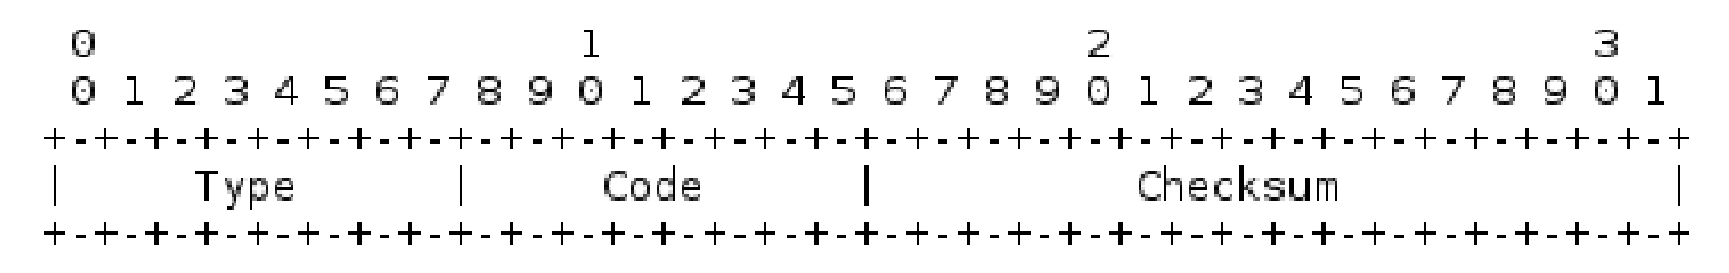
\includegraphics[width=12cm]{./pics/header.eps}
\caption{Champs de l'entête communs à tous les types de message ICMP}
\label{fig:headicmp}
\end{figure}

Le premier champ est celui de type. Il permet, premièrement, de donner le type
du paquet et de l'information à transmettre, et deuxièmement de préciser la
nature des champs qui vont suivre. En effet, comme vu plus haut, les messages
contiennent des champs différents selon le type du message ICMP.  Le deuxième
champ est le code. Il permet de subdiviser le type en donnant des détails plus
précis. Enfin le troisième champ est la somme de contrôle (checksum).
Commençons avec les messages qui possèdent l'ensemble de champs le plus simple.

\begin{figure}[h]
\centering
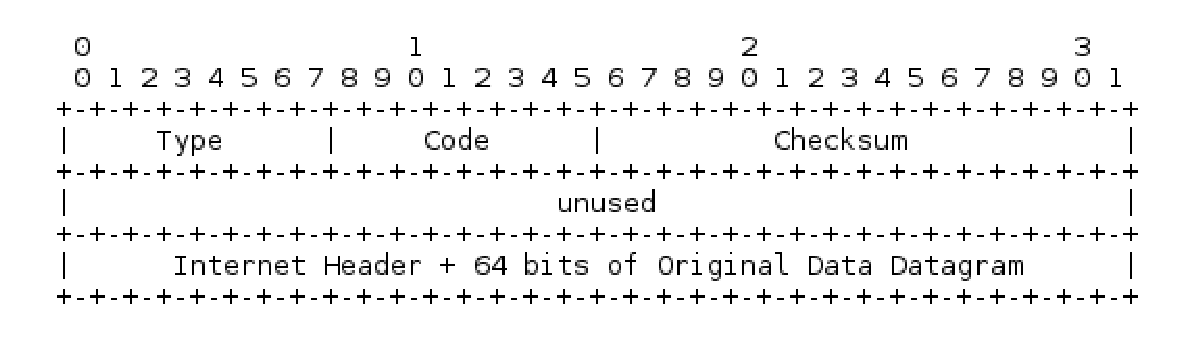
\includegraphics[width=12cm]{./pics/header1.eps}
\caption{Entête des messages de type 3 et 11}
\label{fig:head1icmp}
\end{figure}

Les messages qui utilisent cette organisation sont les messages de type 3 et
11.  Le champ Internet header contient l'entête du paquet qui a provoqué
l'envoie du message ICMP, plus les 64 premiers bits suivant le header. Cela
permet à l'émetteur de retrouver quel paquet à posé problème.

\vspace{1cm}
\textbf{Message de type 3: Unreachable Destination}
Les messages de type 3 sont émis lorsqu'un paquet n'a pas réussi à joindre la
destination (Unreachable destination). Cette erreur peux être dut à plusieurs
facteurs, et les codes permettent de préciser pourquoi le paquet n'a pas pu
rejoindre sa destination.

\paragraph{Code 0: Network Unreachable} Ce code indique que le réseau que
l'hôte essaye d'atteindre n'est pas joignable; ceci étant dut à l'absence de
route vers ce réseau.

\paragraph{Code 1: Host Unreachable} Ce code indique que le réseau à été joint,
mais que le routeur sur ce réseau n'arrive pas à joindre l'hôte à qui délivrer
la trame.

\paragraph{Code 2: Protocole Unreachable} Ce code indique que l'hôte à été
joint, mais que le protocole utilisé n'est pas actif.

\paragraph{Code 3: Port Unreachable} Ce code indique que l'hôte à été joint,
mais que le port utilisé en couche transport n'est pas actif et ne peux donc
être utilisé pour communiquer.

\paragraph{Code 4: Fragmentation needed} Ce code indique que la taille du
paquet dépasse le MTU (Maximum Transmission Unit) et que le flag DF à été mis à
1 dans l'entête IP.  En règle général, si un paquet est plus grand que le MTU,
il doit être fragmenté par le routeur pour être transmis en plusieurs paquets
plus petit. Mais comme le flag DF (Do not Fragment) est mis à 1, le paquet ne
peux être fragmenté. Le routeur émet donc un paquet ICMP de code 4.

Ces codes ont été définis dans la RFC 792, mais depuis d'autre RFC ont ajouté
des codes en plus qui sont utilisés dans des cas plus précis.

\vspace{1cm}
\textbf{Message de type 11: Time Exceeded}
Ce message est envoyé lorsque le TTL d'un paquet à atteint 0. Une autre
utilisation des ces messages est lorsque que le temps de ré-assemblage des
fragments d'un paquet est dépassé. Ces deux cas sont distingué par le code. Ces
messages ont pour destinataire l'hôte qui à envoyé le paquet qui à provoqué
l'erreur.%TODO(vérifier).

\paragraph{Code 0:}
Le code 0 est utilisé pour indiquer que le TTL du paquet posant problème est
arrivé à 0.  Lorsque le TTL d'un paquet arrive à 0, celui-ci est supprimé et un
message ICMP de type 11 et de code 0 est envoyé par le routeur qui à détecté le
problème. Cela permet principalement d'éviter qu'un paquet entre dans une
boucle et qu'il soit relayé à l'infini.

\paragraph{Code 1:} Le code 1 est quant à lui utilisé pour indiquer que l'hôte
n'a pas réussi à réassembler les fragments du paquet IP original dans la limite
de temps prévue à cet effet.


\vspace{1cm}
\textbf{Message de type 5: Redirect Message} Les message de type 5 utilisent
l'entête ci-dessous et servent à faire de la redirection. En effet, lorsqu'un
routeur détecte que le prochain routeur dans lequel va transiter le paquet se
trouve dans le même réseau que l'émetteur de ce paquet, il va envoyer un
message ICMP pour avertir cet hôte (et dans certain cas tous les hôtes sur le
réseau de l'émetteur) qu'il existe un chemin plus court en envoyant directement
les paquets vers le prochain routeur. Ce message ICMP va avoir pour effet de
modifier la table de routage interne à l'émetteur (et dans certain cas tout les
hôtes présent sur le réseau de l'hôte). Concernant le paquet que le premier
routeur à reçu, il va le transmettre vers sa destination.


\begin{figure}[h]
\centering
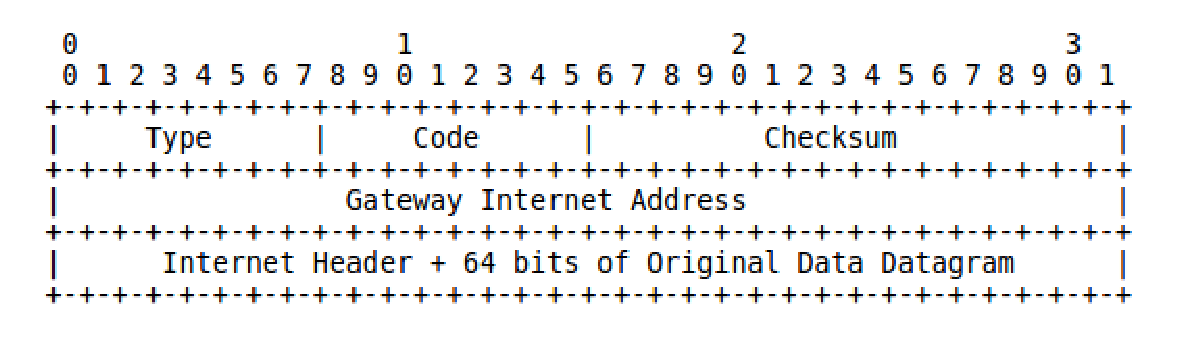
\includegraphics[width=13cm]{./pics/header2.eps}
\caption{Entête des messages de type 5}
\label{fig:head2icmp}
\end{figure}
Le champ Gateway Internet Address contient la l'adresse du routeur auquel il
faut faire transiter le trafique directement pour avoir un chemin de routage
plus court.  Le champ Internet Header contient toujours l'entête du message
ayant provoqué l'envoie du message ICMP plus les 64 bits suivant l'entête. Cela
permet à (aux) hôte(s) de pouvoir modifier leur table de routage en fonction la
destination que cherchait à atteindre le paquet.

\paragraph{Code 0}
Ce code indique que la redirection est adressée à tout les hôtes présent sur le
réseau de l'émetteur du paquet.

\paragraph{Code 1}
Ce code indique que la redirection est adressée à l'émetteur du paquet.

\paragraph{Code 2}
Ce code indique que la redirection est adressée à tout les hôtes présent sur le
réseau de l'émetteur du paquet et aux services.

\paragraph{Code 3} Ce code indique que la redirection est adressée à l'émetteur
du paquet et aux services.

Les messages de code 2 et 3 vont agir sur les services, notamment sur le ToS.

\begin{figure}[h]
\centering
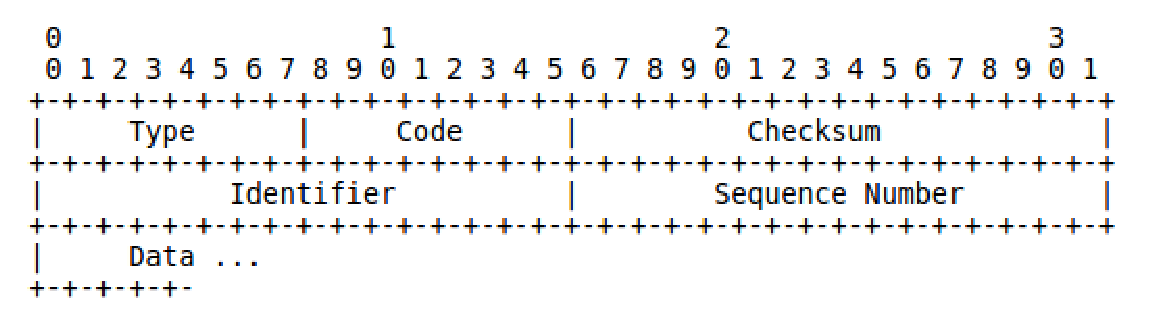
\includegraphics[width=13cm]{./pics/header3.eps}
\caption{Entête des messages de type 0 et 8}
\label{fig:head3icmp}
\end{figure}

\vspace{1cm}
\textbf{Message de type 8 et 0: Echo Request et Reply} Les messages de type 8
et 0 servent à faire des envoies et des renvoies d'information. Ils utilisent
pour cela l'entête ci-dessus. Les messages de type 8 font des envoies
d'informations, appelé echo request. Tandis que les messages de type 0 sont
envoyés en réponse aux echo request et renvoient les informations reçus de
ceux-ci; ils sont appelés echo reply. Etant donnée que les echo reply sont des
réponses aux echo request, l'adresse IP destination des echo reply est
l'adresse IP source des echo request. Ces deux messages peuvent être envoyés et
reçus aussi bien par un hôte que par un routeur. Ce sont notamment les messages
envoyés par la commande {\it ping} qui permettent de vérifier si l'on peux
communiquer avec un hôte ou un routeur.  Les champs Identifier et Sequence
Number aide l'émetteur de l'echo request à associer les echos request qu'il à
envoyés avec les echos reply qu'il à reçus.

\vspace{1cm}
Il y a bien d'autre types et code défini par ICMP, cependant ils sont plus
spécifiques ou devenu obsolètes.


%----------------------------------------------------------------------------------

\subsection{IGMP}
Le protocole IGMP est un autre protocole faisant partit intégrante d'IPv4. Il
permet en effet aux hôtes de communiquer aux routeur mutlicast leur abonnement
à des groupes multicast.  IGMPv2 et IGMPv3 sont les versions les plus utilisées
actuellement. Elles sont respectivement décrient dans le RFC
2236\cite{url-RFC-IGMP2} et RFC 3376\cite{url-RFC-IGMP3}.  Les messages IGMP
sont divisées en trois groupe:
\begin{itemize}
\item Membership Query: Les requêtes d'adhésion: servant aux routeurs pour
faire une demande aux hôtes des groupes auxquels ils sont abonnés.
\item Membership Report: Les rapports d'hôte sur leurs abonnements.
\item Leave Group: Message annonçant l'arrêt d'un abonnement d'un hôte.
\end{itemize}
Tout ces messages sont envoyés avec un TTL de 1, pour éviter que ceci ne
passent d'un réseau à un autre.

\smallbreak
IGMP va donc permettre aux routeurs d'apprendre les groupes d'abonnements des
hôtes qui sont sur le ou les réseaux du routeur. Le routeur dispose d'une liste
des groupes multicast auxquels les hôtes d'un réseau sont connectés, et ceci
pour tout les réseaux auxquels il est connecté.  Pour commencer, le routeur va
envoyer à l'adresse 224.0.0.1, deux (par défaut) Membership Query général à 30
secondes d'intervalles (par défaut).

\smallbreak
Lorsqu'un hôte reçoit un Membership Query, il va initialiser un timer pour
chaque groupe multicast auxquels il appartient. Ces timers sont initialisés
avec un temps aléatoire dont la borne supérieur est spécifié dans le Membership
Query. Ce système de timers permet de ne pas saturer le réseau avec touts les
message IGMP de tout les groupes qui seraient envoyé au même moment.  Lorsque
le timer d'un des abonnements arrive à 0, alors l'hôte émet, en multicast au
groupe en question, un Membership Report.  Si l'hôte reçoit un Membership
Report et que le timer du groupe concerné par le message reçus n'a pas encore
atteint 0, alors l'hôte va arrêter le timer. En effet le routeur sera aux
courant de l'existence du groupe car il aura reçu le même rapport que l'hôte.

\smallbreak
Le protocole IGMP est conçu pour que le routeur sache à quels groupe multicast
sont abonnés les hôte sur les réseaux auxquels il est relié. Cependant le
protocole n'a pas du tout été conçu dans l'optique de fournir la liste des
hôtes avec leurs abonnements.  C'est pour cela qu'une fois que le routeur est
au courant de l'existence d'un groupe, les autre hôtes faisant partie de ce
groupe n'envoie pas de rapport pour ce groupe.

\smallbreak
Lorsque le routeur reçoit un Membership Report il va ajouter le groupe à sa
liste de groupe présent sur le réseau auquel il est connecté. Il va à ce moment
initialiser un timer à 135 secondes (valeur par défaut).  Si il reçoit d'autre
Membership Report pour un groupe existant alors le timer est remis à sa valeur
initiale (de 135 secondes).  Lorsqu'un hôte rejoint un nouveau groupe, il va
émmetre un Unsolicited Membership Report pour s'annoncer dans le groupe, et
ainsi informer le routeur de l'existence de ce groupe ou de la remise à la
valeur initiale du timer.

\smallbreak
Le dernier cas de figure est lorsqu' un hôte veut se désabonner d'un groupe: il
va donc arrêter de traiter les messages à destination du groupe multicast. Si
l'hôte est le dernier de son groupe alors il va envoyer un Leave Group à
l'adresse 224.0.0.2.  Si il n'est pas le dernier, il peux simplement ne rien
faire et se désabonner du groupe, il ne sera plus concerné par les messages à
destination du groupe. Etant donné qu'il y a d'autres membres dans le groupe
ceci s'occuperont de "maintenir le groupe en vie".  En revanche si l'hôte ne
sais pas si il est le dernier hôte dans le groupe rien ne l'empêche d'envoyer
un Leave Group.

Lorsque le routeur reçoit un Leave Group, il sais qu'un membre à quitté le
groupe. Ce qui l'intéresse est de savoir si il y a encore des membres dans le
groupe en question ou si s'est le dernier membre qui vient de quitter le
groupe. Il va pour cela envoyer deux Membership Query spécifiquement au groupe
en question. Si aucune réponse n'est reçut le groupe est considéré comme
n'ayant plus de membre et il est oublier du routeur.  Si jamais les hôte
n'annonçait pas leur retrait du groupe (comme cela à été évoqué plus haut) et
qu'il n'y avait plus d'hôte faisant partit du groupe, alors le groupe serait
considéré sans membre et oublié lorsque le timer du routeur arriverait à 0 pour
le groupe en question.

\smallbreak
Le dernier point pour que tout cela fonctionnent, est qu'il faut que le routeur
envoie régulièrement des Membership Query général pour qu'il maintiennent à
jour sa table des groupe présent sur le réseau, sinon ceux-ci serait oublier
une fois le timer arrivé à expiration.

%----------------------------------------------------------------------------------------


\subsection{DHCP}
Le protocole DHCP (Dynamic Host Configuration Protocol) sert à l'auto-configuration
des interfaces. Plus précisément, il  permet d'attribuer une adresse IP à une
interface et de lui faire parvenir d'autres information essentielle pour le
fonctionnement de l'interface sur le réseau. 

\newpage
La version initiale de DHCP fut décrite dans le RFC 1531\cite{url-RFC-DHCP1},
mais cette version fut rendue obsolète par un autre RFC, lui même rendue
obsolète par le RFC 2131\cite{url-RFC-DHCP2} qui est la dernière version non
obsolète. Voyons comment une interface peut ce configurer auprès d'un serveur
DHCP.

\begin{figure}[h]
\centering
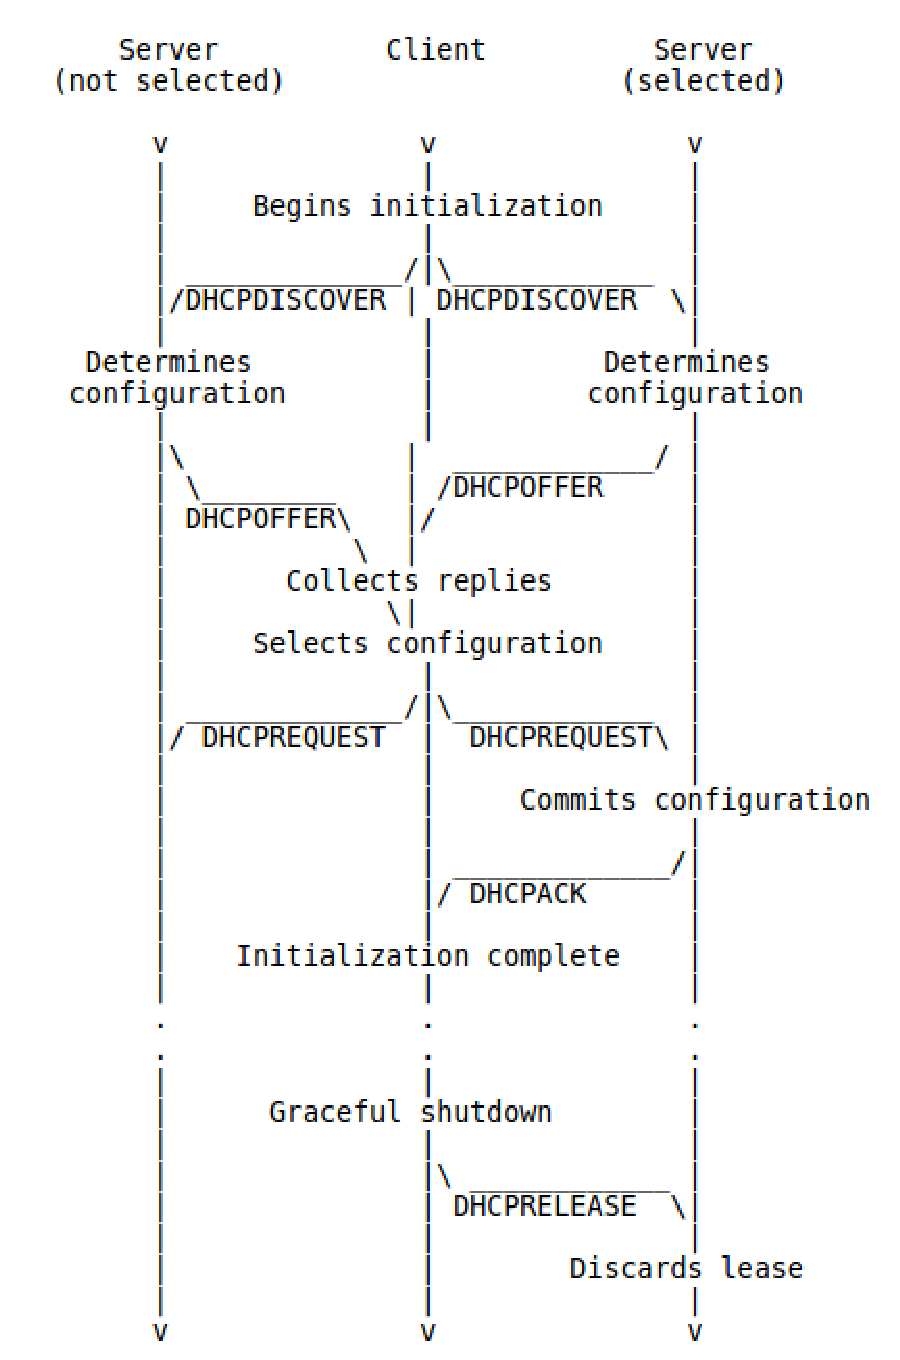
\includegraphics[width=6cm]{./pics/timeline_dhcp.eps}
\caption{Déroulement de la négociation DHCP}
\label{fig:timelinedhcp}
\end{figure}

Lorsqu'une interface, qui n'a pas d'adresse IP, souhaite en recevoir une, elle
va émettre un message DHCPDISCOVERY en broadcast sur son réseau. Des agents
DHCP peuvent faire passer ce message DHCP sur un autre réseau si le serveur
DHCP (qui distribue les adresses) ne se trouve pas sur le même réseau que
l'hôte qui fait la demande.  L'hôte va utiliser comme adresse IP 0.0.0.0.

\smallbreak
Etant donné que le message est envoyé en broadcast, tout les hôtes sur le
réseau vont recevoir le message, et en particulier le ou les serveurs DHCP qui
pourraient s'y trouver. Si cela est le cas, ceux-ci vont répondre avec un
DHCPOFFER. Ce message contient entre autre l'adresse IP proposé pour le client
souhaitant se configurer, ainsi que le masque du réseau. A ce
moment là l'adresse n'est pas encore attribuée et réservée pour l'hôte étant
donnée qu'il peut refuser l'offre et accepter l'offre d'un autre serveur. Si
jamais l'hôte ne reçoit aucun DHCPOFFER, il va ré-émettre un DHCPDISCOVERY. Si
il reçoit un ou plusieurs DHCPOFFER, l'hôte va devoir choisir une configuration
parmis celles qui lui sont proposées. Une fois ce choix fait, il va informer les serveurs DHCP de
son choix à l'aide d'un message DHCPREQUEST émis en broadcast. Ce message va
contenir l'identifiant du serveur DHCP retenu ainsi que la configuration
souhaité par l'hôte (adresse IP et masque du réseau). Ce message peut être
interprété de deux manières différentes selon le serveur:
\begin{itemize}
\item Si ce n'est pas le serveur retenu, il considère le message comme une
déclinaison de l'offre.

\item Si c'est le serveur retenu, il va sortir l'adresse attribuée à l'hôte de la
plage d'adresse libre pour ne plus l'attribuer à un autre hôte. Il va ensuite
émmettre un message DHCPACK contenant la configuration effective de l'hôte avec
notamment: l'adresse IP, le masque du réseau, la durée du bail, l'adresse
de la passerelle par défaut et l'adresse du serveur DNS.  Si pour quelque
raisons que ce soit le serveur n'est pas capable d'attribuer l'adresse proposée dans l'offre
(par exemple si l'adresse à été attribuée entre temps), le serveur émet un
DHCPNAK pour avertir l'hôte que l'adresse n'est plus disponible. L'hôte devra
alors recommencer la procédure pour obtenir une configuration.
\end{itemize}

\smallbreak
Enfin si le serveur ne reçoit pas de message DHCPREQUEST, la procédure
s'arrêtera à ce moment et l'adresse n'étant pas encore attribuée à l'hôte elle
reste disponible pour être attribuée à d'autre hôte. 

\smallbreak
Arrive la dernière étape.
Si l'hôte reçois un message DHCPACK, il peux prendre en compte la
configuration (adresse IP, masque du réseau, DNS, passerelle par défaut et
durée de bail). Il va effectuer une dernière vérification pour s'assurer que
l'adresse qui lui à été attribué est bien unique sur le réseau pour éviter
d'avoir deux hôte avec la même adresse. Il va pour cela utilisé le protocole
ARP et la méthode de vérification vu plus haut. Si jamais l'adresse est déjà
utilisé par un autre hôte, il va envoyer un message DHCPDECLINE au serveur DHCP
pour lui indiquer qu'il n'utilisera pas la configuration proposée par celui-ci,
et il va recommencer la procédure pour pouvoir obtenir une nouvelle
configuration.

\smallbreak
Si jamais l'adresse proposé par le serveur est unique sur le réseau, la
configuration est terminé et l'hôte peut utiliser l'adresse (durant la durée du
bail de celle-ci).  Dernier cas possible, si jamais le l'hôte ne reçoit pas de
DHCPACK ou de DHCPNAK, il va réémettre le message DHCPREQUEST pour espérer
recevoir une réponse du serveur.

\smallbreak
Tout au fil des différents messages échangés, le client est identifié grâce au
champ client identifier, et le serveur grâce au champ server identifier.

L'hôte est donc configuré et peut utiliser son adresse. Cependant, il ne peut
l'utiliser que durant la durée de son bail. Une fois le bail expiré, l'hôte ne
peux plus utiliser son adresse. Lorsque l'hôte a reçu le message DHCPACK du
serveur, celui-ci lui a transmis la durée du bail. De cette durée, l'hôte va
en extraire deux temps noté T1 et T2. T1 correspond à la moitié de la durée du
bail et T2 à 0.875 fois la durée du bail. Ces temps sont exprimés de manière relatif
étant donnée que les horloges du serveur et de l'hôte ne sont pas
synchronisées.  Une fois que l'hôte à atteint le temps T1, il va chercher à
contacter le serveur qui lui à attribué sa configuration avec un message
DHCPREQUEST pour étendre la durée de son bail. Ce message est émis de manière
unicast. A ce moment l'hôte est entré en état RENEWING. Si l'hôte reçoit un
message DHCPACK du serveur lui accordant un prolongement de la durée de son
bail, alors il va sommer le temps qu'il avait insérer dans le DHCPREQUEST avec
la durée accordée par le serveur et qui se trouve dans le message DHCPACK.
L'hôte retourne dans l'état BOUND. Cependant l'hôte n'est pas obligé d'attendre
T1 pour pouvoir étendre son bail.  Si jamais l'hôte ne reçoit pas de réponse
DHCPACK avant l'arrivé de T2, il passe en état REBINDING. A ce moment il va
émettre un DHCPREQUEST en broadcast pour espérer pouvoir étendre son bail
auprès de n'importe quel serveur DHCP. Pour parer aux éventuels cas de perte de
DHCPREQUEST, l'hôte va renvoyer un message une fois la moitié de la durée entre
T1 et T2 passé, en état RENEWING; et une fois la moitié de la durée entre T2 et
la fin du baille , en état REBINDING (et avec un minimum de temps de 60
secondes).  Si malgré tout, la durée du bail venait à expirer, alors l'hôte ne
posséderait plus de configuration réseau et ne pourrait plus communiquer avec
d'autre hôtes. Il rentre alors en état INIT; il doit alors recommencer la
procédure pour obtenir une configuration.

\smallbreak
Cependant,dans ce cas comme dans d'autre, l'hôte peut ré-utiliser une
configuration précédemment utilisée. Cela permet de raccourcir la négociation
entre l'hôte et le serveur DHCP. L'hôte va directement commencer la négociation
en faisant un DHCPREQUEST en broadcast et contenant la configuration qu'il
souhaite ré-utiliser. Le serveur concerné par l'attribution antérieur de la
configuration va donc accepter la demande de l'hôte à l'aide d'un DHCPACK ou la
refuser, si la demande n'est pas correct ou si l'adresse est utilisé par un
autre hôte, à l'aide d'un DHCPNAK.  Cette négociation se fait de manière
similaire à une négociation complète, elle a juste été raccourci en enlevant
quelques étapes non indispensables.

\begin{figure}[h]
\centering
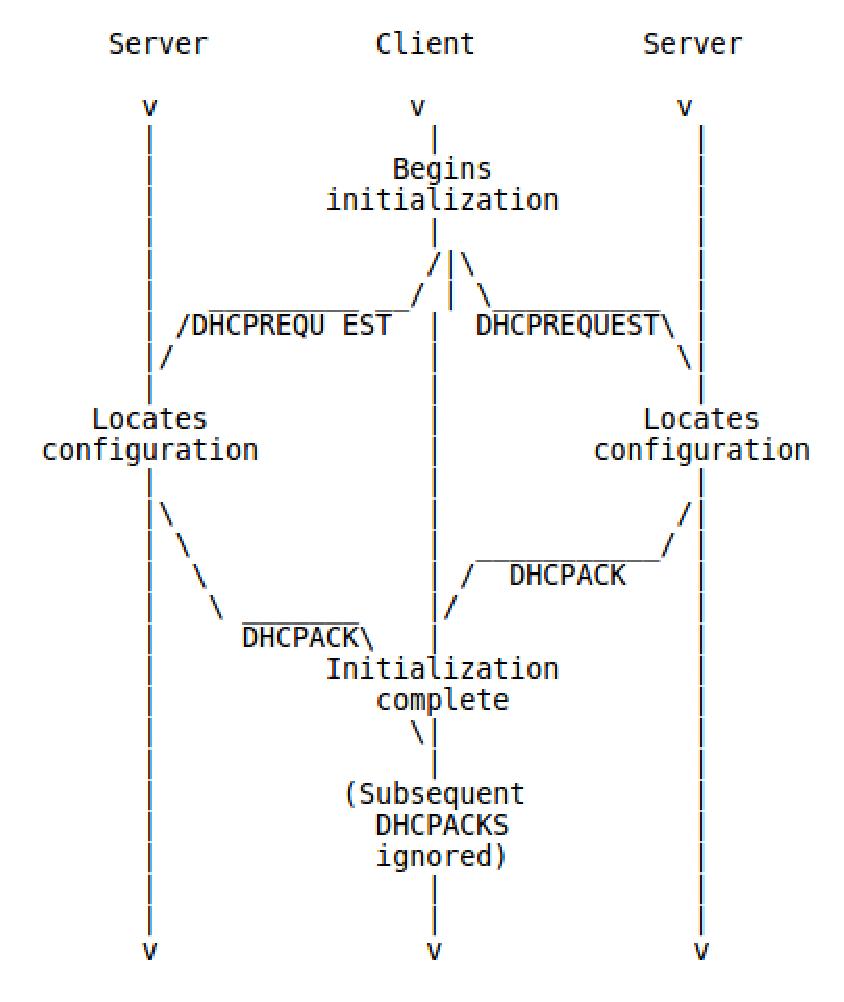
\includegraphics[width=6cm]{./pics/timeline_dhcp_reuse_add.eps}
\caption{Déroulement de la négociation DHCP pour la réutilisation d'une configuration}
\label{fig:timelinedhcpreuseadd}
\end{figure}

%---------------------------------------------------------------------------------

\subsection{PMTU discovery}
Le protocole PMTU discovery (Path MTU discovery) décrit dans le RFC
1191\cite{url-RFC-PMTU}, permet de trouver le plus petit MTU d'un chemin entre
l'émetteur et le récepteur. Cela permet d'éviter la fragmentation des paquets
IP ce qui permet entre autre de soulager la charge des routeurs.  L'hôte
souhaitant connaître le plus petit MTU pour un chemin vers autre hôte va
envoyer un paquet avec un certain MTU et en plaçant le bit DF de l'entête sur 1
pour éviter la fragmentation du paquet. Ainsi si le MTU est trop grand à un
moment donné du chemin, le routeur ne pourra pas fragmenter le paquet mais ne
pourra non plus pas transmettre le paquet en l'état. Il va alors détruire le
paquet, et émettre un message ICMP de type 3 et de code 4 vers la source du
paquet, signalant que la destination n'est pas joignable, et que cela est dut à
un paquet nécessitant une fragmentation or celle-ci est interdite. Le MTU est
donc trop élevé. Le message ICMP contient le MTU qu'il faut passé le routeur.
L'émetteur va alors créer un nouveau paquet avec le nouveau MTU. Il fera cela
autant de fois que cela est nécessaire pour déterminer le MTU du chemin.

\subsection{DNS}
Le protocole DNS (Domain Name System) permet de faire de la résolution
d'adresse.  Cela est permis grâce à des échanges avec un ou plusieurs serveur DNS.
Un serveur DNS va faire de la traduction de nom de domaine, notamment en adresse IP. Pour
simplifier, le nom de domaine, facilement retenu par un être humain va être
traduit en adresse IP pour être utilisée par l'ordinateur.  Nous n'aborderons
pas plus le fonctionnement de DNS car s'est un protocole de couche application
et qu'il n'est pas essentiel au fonctionnement d'IPv4. Cependant il reste
essentiel dans l'utilisation d'Internet, aujourd'hui, par des êtres humains.
